% Options for packages loaded elsewhere
% Options for packages loaded elsewhere
\PassOptionsToPackage{unicode}{hyperref}
\PassOptionsToPackage{hyphens}{url}
\PassOptionsToPackage{dvipsnames,svgnames,x11names}{xcolor}
%
\documentclass[
  english,
  letterpaper,
  DIV=11,
  numbers=noendperiod]{scrartcl}
\usepackage{xcolor}
\usepackage{amsmath,amssymb}
\setcounter{secnumdepth}{5}
\usepackage{iftex}
\ifPDFTeX
  \usepackage[T1]{fontenc}
  \usepackage[utf8]{inputenc}
  \usepackage{textcomp} % provide euro and other symbols
\else % if luatex or xetex
  \usepackage{unicode-math} % this also loads fontspec
  \defaultfontfeatures{Scale=MatchLowercase}
  \defaultfontfeatures[\rmfamily]{Ligatures=TeX,Scale=1}
\fi
\usepackage{lmodern}
\ifPDFTeX\else
  % xetex/luatex font selection
\fi
% Use upquote if available, for straight quotes in verbatim environments
\IfFileExists{upquote.sty}{\usepackage{upquote}}{}
\IfFileExists{microtype.sty}{% use microtype if available
  \usepackage[]{microtype}
  \UseMicrotypeSet[protrusion]{basicmath} % disable protrusion for tt fonts
}{}
\makeatletter
\@ifundefined{KOMAClassName}{% if non-KOMA class
  \IfFileExists{parskip.sty}{%
    \usepackage{parskip}
  }{% else
    \setlength{\parindent}{0pt}
    \setlength{\parskip}{6pt plus 2pt minus 1pt}}
}{% if KOMA class
  \KOMAoptions{parskip=half}}
\makeatother
% Make \paragraph and \subparagraph free-standing
\makeatletter
\ifx\paragraph\undefined\else
  \let\oldparagraph\paragraph
  \renewcommand{\paragraph}{
    \@ifstar
      \xxxParagraphStar
      \xxxParagraphNoStar
  }
  \newcommand{\xxxParagraphStar}[1]{\oldparagraph*{#1}\mbox{}}
  \newcommand{\xxxParagraphNoStar}[1]{\oldparagraph{#1}\mbox{}}
\fi
\ifx\subparagraph\undefined\else
  \let\oldsubparagraph\subparagraph
  \renewcommand{\subparagraph}{
    \@ifstar
      \xxxSubParagraphStar
      \xxxSubParagraphNoStar
  }
  \newcommand{\xxxSubParagraphStar}[1]{\oldsubparagraph*{#1}\mbox{}}
  \newcommand{\xxxSubParagraphNoStar}[1]{\oldsubparagraph{#1}\mbox{}}
\fi
\makeatother


\usepackage{longtable,booktabs,array}
\usepackage{calc} % for calculating minipage widths
% Correct order of tables after \paragraph or \subparagraph
\usepackage{etoolbox}
\makeatletter
\patchcmd\longtable{\par}{\if@noskipsec\mbox{}\fi\par}{}{}
\makeatother
% Allow footnotes in longtable head/foot
\IfFileExists{footnotehyper.sty}{\usepackage{footnotehyper}}{\usepackage{footnote}}
\makesavenoteenv{longtable}
\usepackage{graphicx}
\makeatletter
\newsavebox\pandoc@box
\newcommand*\pandocbounded[1]{% scales image to fit in text height/width
  \sbox\pandoc@box{#1}%
  \Gscale@div\@tempa{\textheight}{\dimexpr\ht\pandoc@box+\dp\pandoc@box\relax}%
  \Gscale@div\@tempb{\linewidth}{\wd\pandoc@box}%
  \ifdim\@tempb\p@<\@tempa\p@\let\@tempa\@tempb\fi% select the smaller of both
  \ifdim\@tempa\p@<\p@\scalebox{\@tempa}{\usebox\pandoc@box}%
  \else\usebox{\pandoc@box}%
  \fi%
}
% Set default figure placement to htbp
\def\fps@figure{htbp}
\makeatother



\ifLuaTeX
\usepackage[bidi=basic]{babel}
\else
\usepackage[bidi=default]{babel}
\fi
% get rid of language-specific shorthands (see #6817):
\let\LanguageShortHands\languageshorthands
\def\languageshorthands#1{}
\ifLuaTeX
  \usepackage[english]{selnolig} % disable illegal ligatures
\fi


\setlength{\emergencystretch}{3em} % prevent overfull lines

\providecommand{\tightlist}{%
  \setlength{\itemsep}{0pt}\setlength{\parskip}{0pt}}



 


\KOMAoption{captions}{tableheading}
\makeatletter
\@ifpackageloaded{tcolorbox}{}{\usepackage[skins,breakable]{tcolorbox}}
\@ifpackageloaded{fontawesome5}{}{\usepackage{fontawesome5}}
\definecolor{quarto-callout-color}{HTML}{909090}
\definecolor{quarto-callout-note-color}{HTML}{0758E5}
\definecolor{quarto-callout-important-color}{HTML}{CC1914}
\definecolor{quarto-callout-warning-color}{HTML}{EB9113}
\definecolor{quarto-callout-tip-color}{HTML}{00A047}
\definecolor{quarto-callout-caution-color}{HTML}{FC5300}
\definecolor{quarto-callout-color-frame}{HTML}{acacac}
\definecolor{quarto-callout-note-color-frame}{HTML}{4582ec}
\definecolor{quarto-callout-important-color-frame}{HTML}{d9534f}
\definecolor{quarto-callout-warning-color-frame}{HTML}{f0ad4e}
\definecolor{quarto-callout-tip-color-frame}{HTML}{02b875}
\definecolor{quarto-callout-caution-color-frame}{HTML}{fd7e14}
\makeatother
\makeatletter
\@ifpackageloaded{caption}{}{\usepackage{caption}}
\AtBeginDocument{%
\ifdefined\contentsname
  \renewcommand*\contentsname{Table of contents}
\else
  \newcommand\contentsname{Table of contents}
\fi
\ifdefined\listfigurename
  \renewcommand*\listfigurename{List of Figures}
\else
  \newcommand\listfigurename{List of Figures}
\fi
\ifdefined\listtablename
  \renewcommand*\listtablename{List of Tables}
\else
  \newcommand\listtablename{List of Tables}
\fi
\ifdefined\figurename
  \renewcommand*\figurename{Figure}
\else
  \newcommand\figurename{Figure}
\fi
\ifdefined\tablename
  \renewcommand*\tablename{Table}
\else
  \newcommand\tablename{Table}
\fi
}
\@ifpackageloaded{float}{}{\usepackage{float}}
\floatstyle{ruled}
\@ifundefined{c@chapter}{\newfloat{codelisting}{h}{lop}}{\newfloat{codelisting}{h}{lop}[chapter]}
\floatname{codelisting}{Listing}
\newcommand*\listoflistings{\listof{codelisting}{List of Listings}}
\makeatother
\makeatletter
\makeatother
\makeatletter
\@ifpackageloaded{caption}{}{\usepackage{caption}}
\@ifpackageloaded{subcaption}{}{\usepackage{subcaption}}
\makeatother
\usepackage{bookmark}
\IfFileExists{xurl.sty}{\usepackage{xurl}}{} % add URL line breaks if available
\urlstyle{same}
\hypersetup{
  pdftitle={Model selection for Markov random fields on graphs under a mixing condition},
  pdfauthor={Magno Severino},
  pdflang={en},
  colorlinks=true,
  linkcolor={blue},
  filecolor={Maroon},
  citecolor={Blue},
  urlcolor={Blue},
  pdfcreator={LaTeX via pandoc}}


\title{Model selection for Markov random fields on graphs under a mixing
condition}
\usepackage{etoolbox}
\makeatletter
\providecommand{\subtitle}[1]{% add subtitle to \maketitle
  \apptocmd{\@title}{\par {\large #1 \par}}{}{}
}
\makeatother
\subtitle{XVII CLAPEM}
\author{Magno Severino}
\date{2026-03-06}
\begin{document}
\maketitle


\subsection{Agenda}\label{agenda}

\subsection{Vector-Valued Stochastic
Processes}\label{vector-valued-stochastic-processes}

\begin{itemize}
\item
  \(\bf X^{(i)} = \big(X_1^{(i)}, X_2^{(i)}, \dots, X_d^{(i)}\big).\)
\item
  \(X_v^{(i)} \in A,\) \(A\) a finite alphabet.
\item
  Process \(\bf X = \{X^{(i)}: -\infty<i<\infty\}.\)
\item
  We assume the process \(\bf X\) has an underlying graph
  \(G^* = (V, E^*).\)
\end{itemize}

\begin{center}

\includegraphics[width=6.94792in,height=4.16667in]{slides_files/figure-pdf/unnamed-chunk-1-1.pdf}
\end{center}

\begin{tcolorbox}[enhanced jigsaw, breakable, title=\textcolor{quarto-callout-important-color}{\faExclamation}\hspace{0.5em}{Important}, colframe=quarto-callout-important-color-frame, toptitle=1mm, leftrule=.75mm, opacitybacktitle=0.6, titlerule=0mm, bottomrule=.15mm, opacityback=0, left=2mm, bottomtitle=1mm, arc=.35mm, colback=white, colbacktitle=quarto-callout-important-color!10!white, coltitle=black, rightrule=.15mm, toprule=.15mm]

Unlike lattice models (regular grids), the graph \(G^*\) in this
framework is general and non-homogeneous.

\end{tcolorbox}

\subsection{Vector-Valued Stochastic
Processes}\label{vector-valued-stochastic-processes-1}

\begin{itemize}
\item
  \(\bf X^{(i)} = \big(X_1^{(i)}, X_2^{(i)}, \dots, X_d^{(i)}\big).\)
\item
  \(X_v^{(i)} \in A,\) \(A\) a finite alphabet.
\item
  Process \(\bf X = \{X^{(i)}: -\infty<i<\infty\}.\)
\item
  We assume the process \(\bf X\) has an underlying graph
  \(G^* = (V, E^*).\)
\end{itemize}

\begin{center}

\includegraphics[width=6.94792in,height=4.16667in]{slides_files/figure-pdf/unnamed-chunk-2-1.pdf}
\end{center}

\begin{tcolorbox}[enhanced jigsaw, breakable, title=\textcolor{quarto-callout-important-color}{\faExclamation}\hspace{0.5em}{Important}, colframe=quarto-callout-important-color-frame, toptitle=1mm, leftrule=.75mm, opacitybacktitle=0.6, titlerule=0mm, bottomrule=.15mm, opacityback=0, left=2mm, bottomtitle=1mm, arc=.35mm, colback=white, colbacktitle=quarto-callout-important-color!10!white, coltitle=black, rightrule=.15mm, toprule=.15mm]

Unlike lattice models (regular grids), the graph \(G^*\) in this
framework is general and non-homogeneous.

\end{tcolorbox}

\subsection{Why go beyond the I.I.D.
assumption?}\label{why-go-beyond-the-i.i.d.-assumption}

Most traditional graphical model techniques assume that observations
\(\mathbf{X}^{(1)}, \mathbf{X}^{(2)}, \dots\) are Independent and
Identically Distributed (i.i.d.).

However, in real-world scenarios, the independence assumption is often
too restrictive:

\begin{itemize}
\tightlist
\item
  \textbf{EEG Time Series}: Neural dependencies evolve over time.
\item
  \textbf{River Stream Flow}: Successive observations exhibit
  hydrological dependence.
\item
  \textbf{Financial Markets}: Daily indices show significant
  autocorrelation and mixing properties.
\end{itemize}

\textbf{Our Proposal}: A global model selection criterion that ensures
consistency even under \textbf{polynomial mixing conditions}.

\subsection{Objectives of the
research}\label{objectives-of-the-research}

\begin{itemize}
\item
  \textbf{Proposal}: Method to estimate the graph of conditional
  dependencies for multivariate stochastic processes with mixing
  conditions.
\item
  \textbf{Aim}: combine and generalize previous works,

  \begin{itemize}
  \item
    Leonardi et al.~(2021): method assumes decomposition into subvectors
    with immediate neighbor dependencies,
  \item
    Leonardi et al.~(2023): estimator of neighborhood of each vertex for
    iid data.
  \end{itemize}
\end{itemize}

. . .

\begin{itemize}
\item
  \textbf{Proposed solution}: penalized pseudo-likelihood criterion for
  entire graph estimation for multivariate processes with mixing
  conditions.
\item
  \textbf{Key advantages}:

  \begin{itemize}
  \tightlist
  \item
    Handles non-iid data (mixing condition),
  \item
    Provides a global estimation approach.
  \end{itemize}
\end{itemize}

\subsection{Mixing Condition}\label{mixing-condition}

\begin{itemize}
\tightlist
\item
  \(X^{(i:j)}\) denote the sequence of vectors
  \(X^{(i)}, X^{(i+1)}, \ldots, X^{(j)}.\)
\end{itemize}

O processo satisfaz uma condição de mixing com taxa \(\psi(\ell)\) se a
dependência entre o passado (\(X^{(1:m)}\)) e o futuro
(\(X^{(n:n+k-1)}\)) decai conforme a distância \(n-m\) aumenta:

\begin{equation}\phantomsection\label{eq-mixing}{
\Bigl| \mathbb P (X_{future} | X_{past}) - \mathbb P (X_{future}) \Bigr| \leq \psi(n-m) \mathbb P(X_{future})
}\end{equation}

\subsection{Empirical Probabilities}\label{empirical-probabilities}

The stationary distribution of the process \(\pi\) is unknown, we must
estimate it from the data.

Assume we observe a sample of size \(n\) of the process, denoted by
\(\{x^{(i)}\colon i=1,\dots,n\}\). Then, for any \(W\subset V\) and any
\(a_W\in A^{W}\), \begin{equation*}
    \widehat{\pi}(a_W)  = \frac{N(a_W)}{n}.
\end{equation*}

If \(\:\widehat\pi(a_W)>0\), \begin{equation*}
    \widehat\pi(a_{W'}|a_{W})  = \frac{\widehat\pi(a_{W'\cup W})}{\widehat\pi(a_{W})}\,,
\end{equation*} for two disjoint subsets \(W,W'\subset V\) and
configurations \(a_W\in A^W, a_{W'}\in A^{W'}\).

\subsection{Empirical Probabilities}\label{empirical-probabilities-1}

Given a graph \(G=(V,E),\) define
\[G(v) = \big\{u \in V: (u,v) \in E \big\},\] for \(v \in V,\) the set
of neighbors of \(v\) in graph \(G.\)

Then we can compute \begin{equation*}
    \widehat\pi(a_v|a_{G(v)})  = \frac{\widehat\pi(a_{\{v\}\cup G(v)})}{\widehat\pi(a_{G(v)})}.
\end{equation*}

\subsection{Graph Estimator}\label{graph-estimator}

Given any graph \(G\) and a sample of the process, we define the
pseudo-likelihood function by
\begin{equation}\phantomsection\label{eq-def-lhat}{
\widehat L(G) \;=\;  \prod_{i=1}^n \:\prod_{v \in V}  \widehat\pi(x^{(i)}_v | x^{(i)}_{G(v)})\,.
}\end{equation}

Applying the logarithm we can write expression above as
\begin{equation}\phantomsection\label{eq-log-pseudo}{
\log \widehat L(G) = \sum_{v \in V} \sum_{(a_v\in A)} \sum_{a_{G(v)}\in A^{|G(v)|}} N(a_v,a_{G(v)})\log \widehat\pi(a_v|a_{G(v)})
}\end{equation}

. . .

The regularized graph estimator is given by

\[
  \widehat G = \underset{G}{\arg\max}\Big\{\log \widehat L(G) - \lambda_n \sum_{v \in V} |A|^{|G(v)|}\Big\} \,.
\]

\subsection{Consistency Theorem}\label{consistency-theorem}

\textbf{Theorem 10:} Assume the process
\(\{X^{(i)}: i \in \mathbb{Z}\}\) satisfies the mixing condition
presented before with \(\psi(\ell) = O(1/\ell^{1+\epsilon})\) for some
\(\epsilon>0.\) Then, by taking \(\lambda_n = c \log n,\) we have that
\begin{equation*}
  \widehat G = \underset{G}{\arg\max}\Big\{\log \widehat L(G) - \lambda_n \sum_{v \in V} |A|^{|G(v)|}\Big\}
\end{equation*} satisfies \(\widehat G=G^*\) eventually almost surely as
\(n\to \infty.\)

\subsection{Algorithms for estimation}\label{algorithms-for-estimation}

The objective is to find the optimal graph by maximizing the regularized
log-pseudo-likelihood function:

\[H(G) = \log \widehat L(G) - \lambda_n \sum_{v \in V} |A|^{|G(v)|}.\]

\paragraph{Implemented Search
Strategies}\label{implemented-search-strategies}

\begin{itemize}
\tightlist
\item
  \textbf{Exact Algorithm}: Performs an exhaustive search over the set
  of all possible simple graphs \(\mathcal{G}\)Computational complexity:
  \(2^{d(d-1)/2}\).
\item
  \textbf{Stepwise (Forward/Backward)}: Heuristic approach that adds or
  removes edges based on local improvements of \(H(G)\).
\item
  \textbf{Simulated Annealing}: A stochastic global search metaheuristic
  used to approximate the estimator in high-dimensional spaces.
\end{itemize}

\href{https://github.com/magnotairone/MixingGraph/}{The
\texttt{MixingGraph} Package}

\begin{center}
\includegraphics[width=1.35417in,height=\textheight,keepaspectratio]{slides_files/mediabag/logo.png}
\end{center}

Comprehensive tools for estimating the graph \(\hat{G}\), executing
search algorithms, and ensuring reproducible results.

\section{Application to real data}\label{application-to-real-data}

\subsection{São Francisco River Data}\label{suxe3o-francisco-river-data}

\begin{center}
\pandocbounded{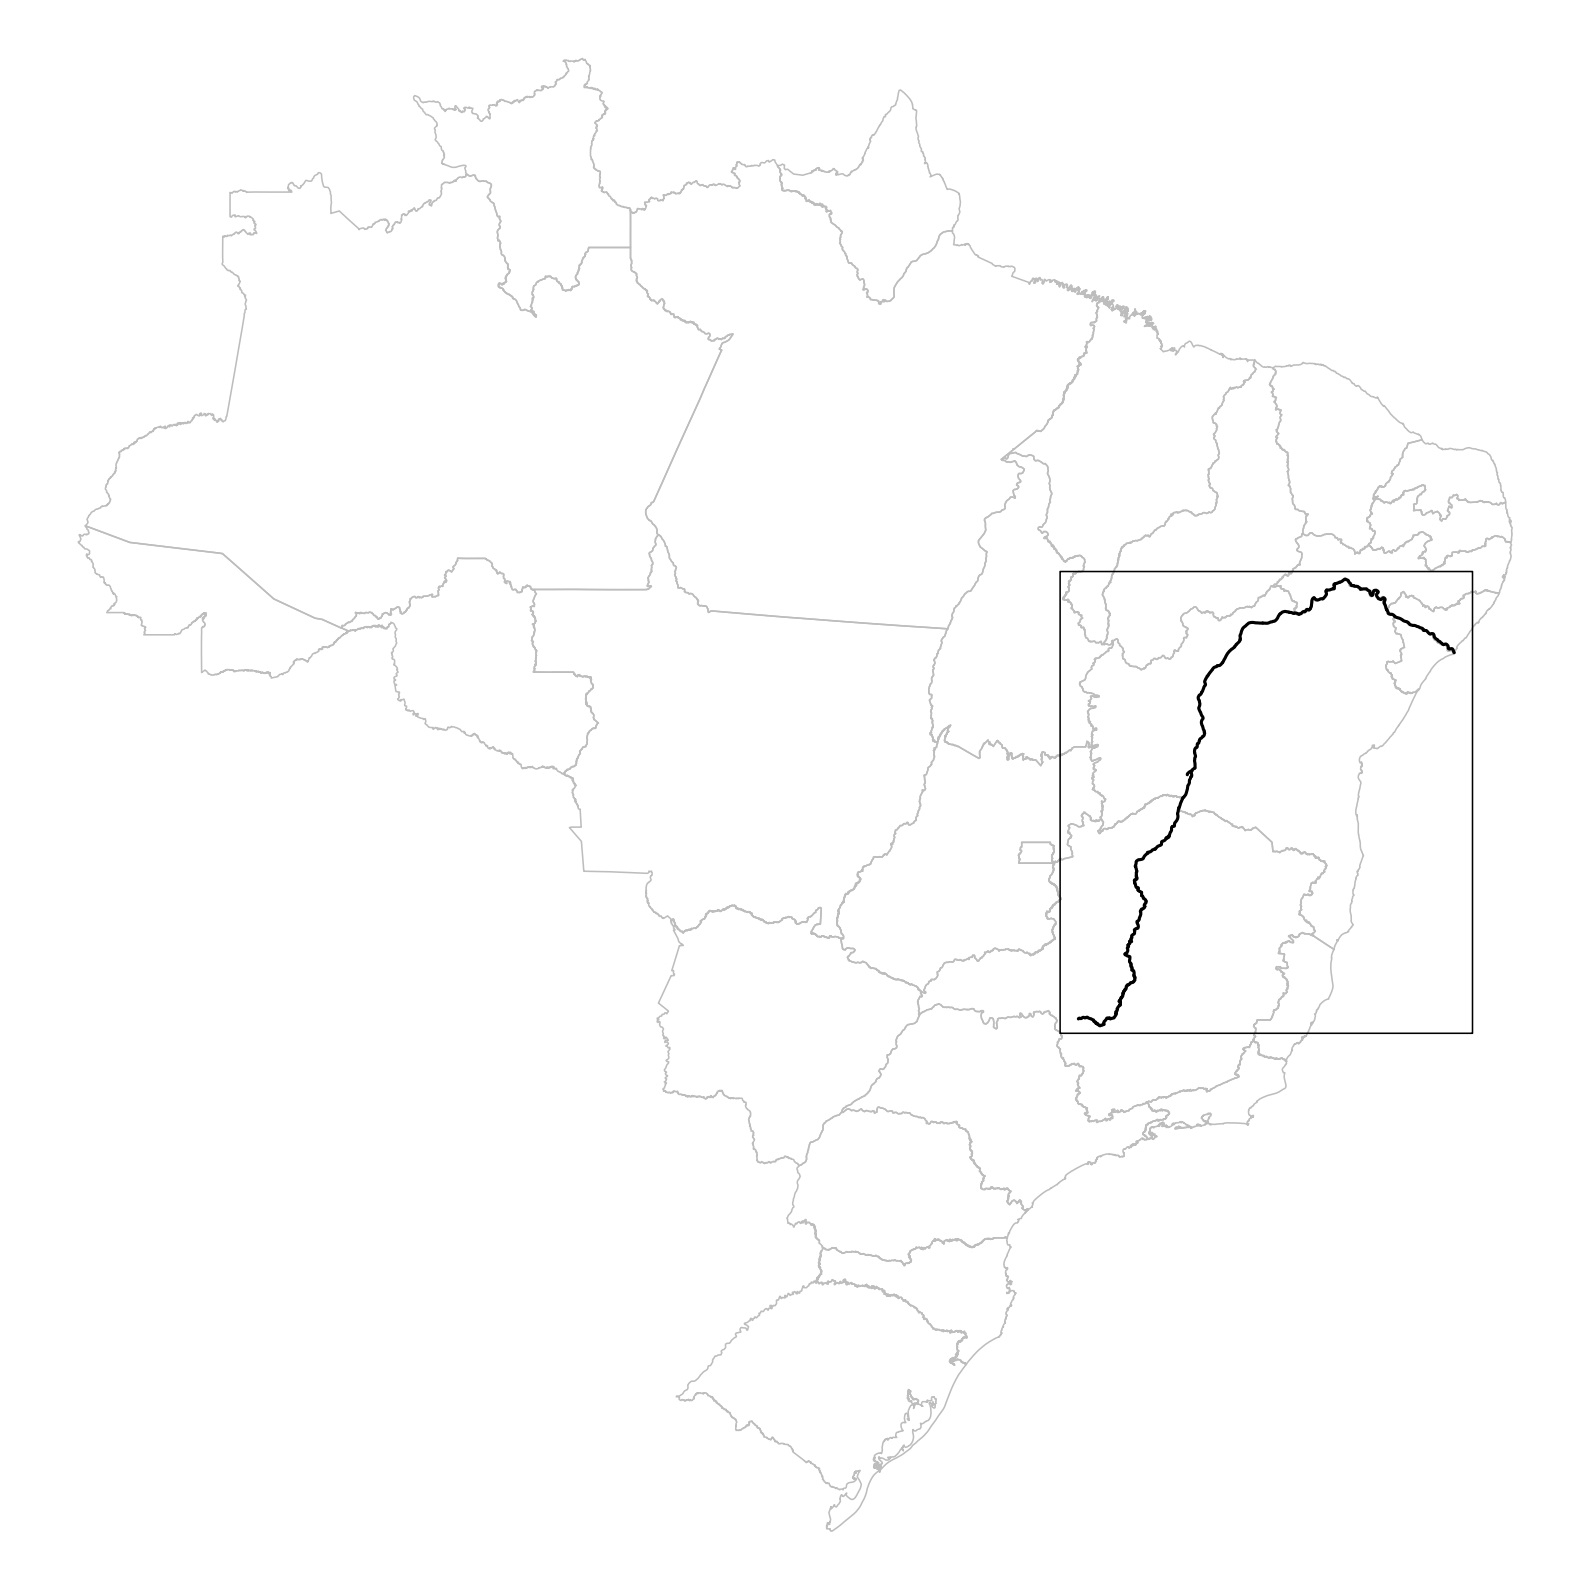
\includegraphics[keepaspectratio]{images/sim/SF_map.jpg}}
\end{center}

\begin{center}
\pandocbounded{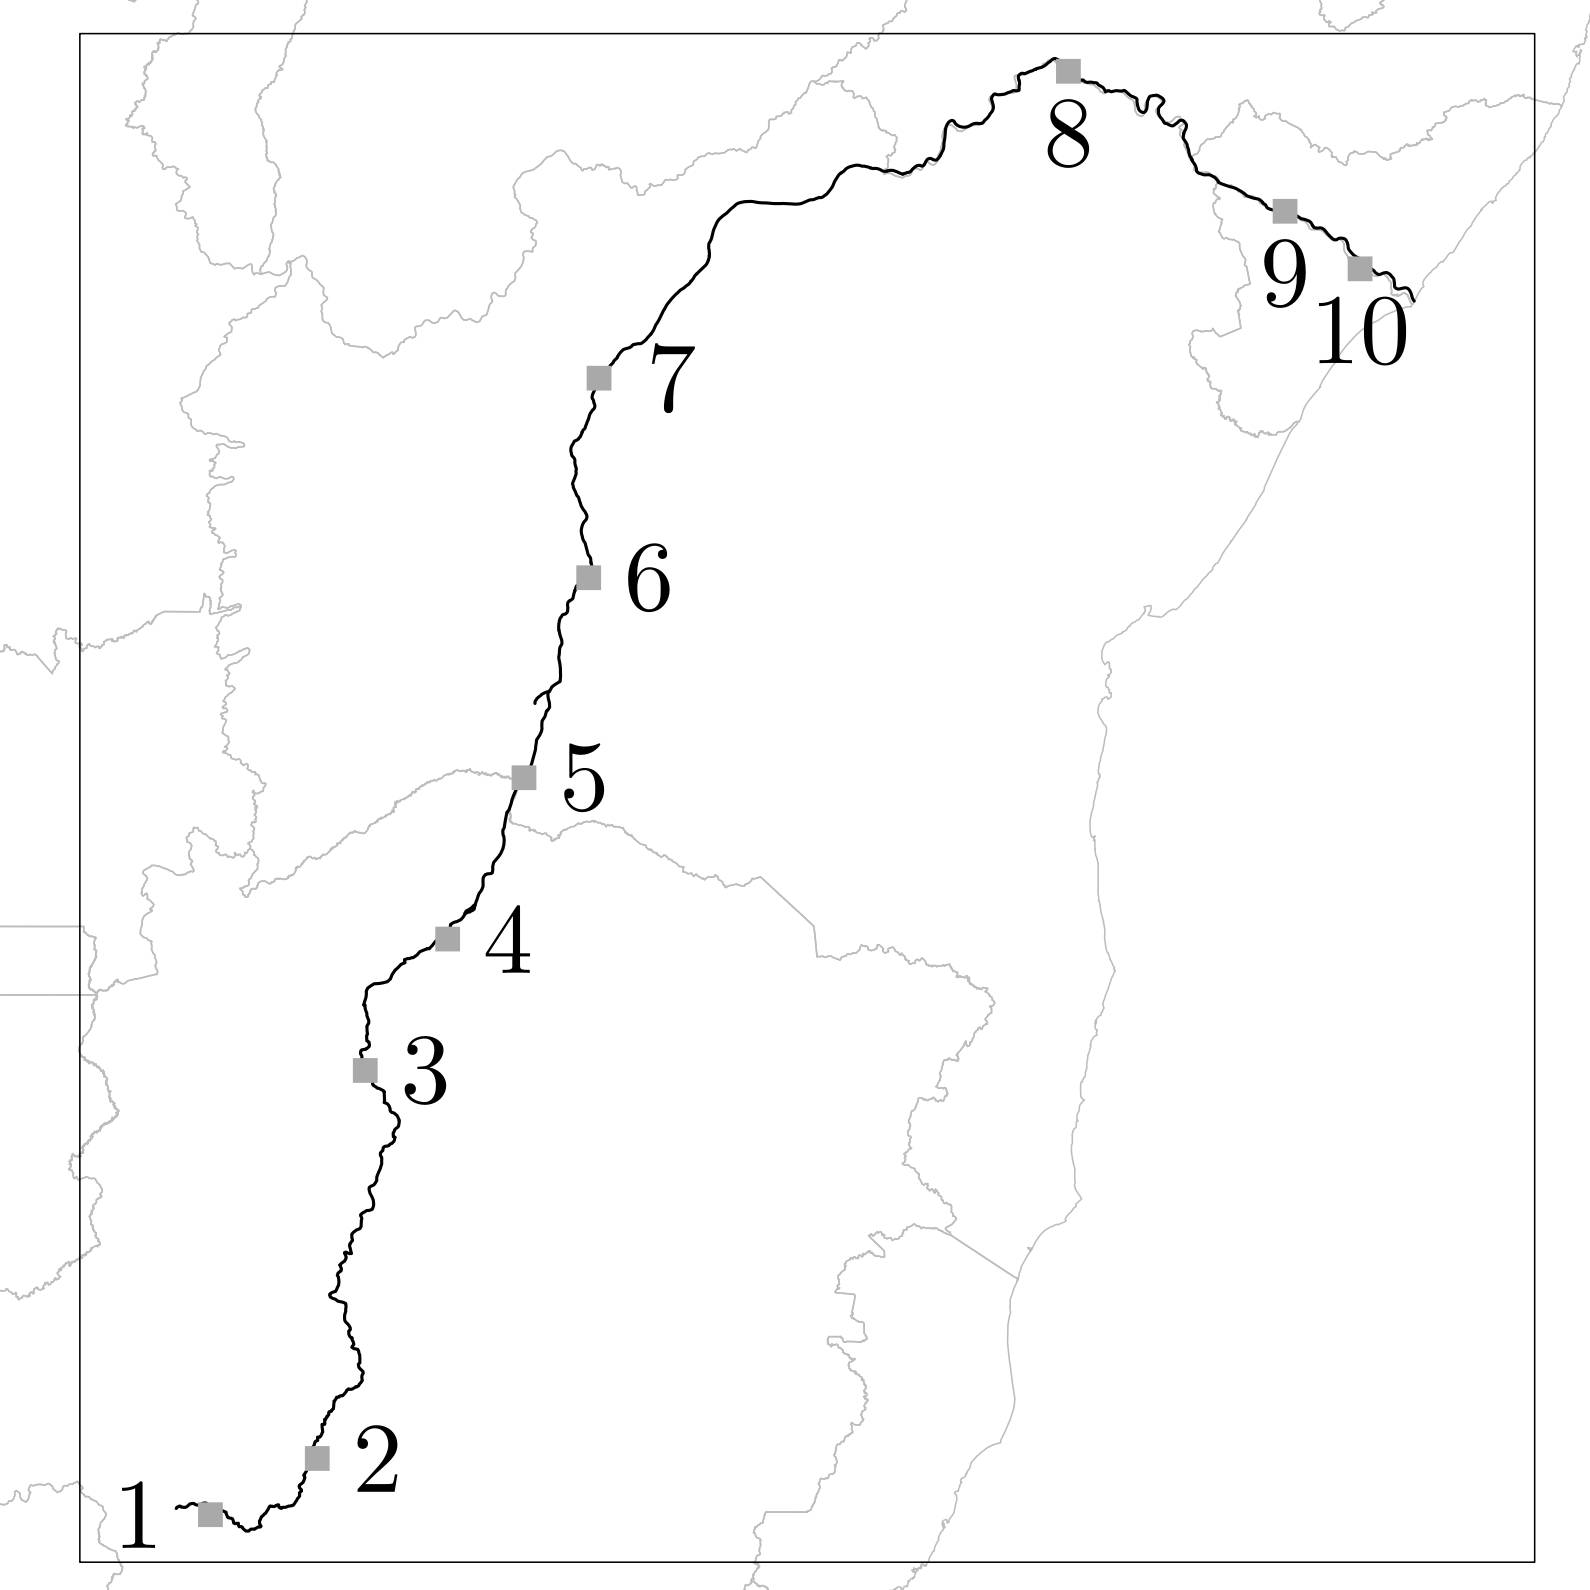
\includegraphics[keepaspectratio]{images/sim/SF_stations.jpg}}
\end{center}

\subsection{São Francisco River
Data}\label{suxe3o-francisco-river-data-1}

\begin{itemize}
\item
  Water volume measured at \(d\) stations along the river's course.
\item
  Stations denoted as \(X_{u}\), where \(u = 1, \ldots, d\).
\item
  Vector \(\mathbf{X}\) observed at discrete time intervals (10-day
  mean).
\item
  Each observation denoted as
  \(\mathbf{X}^{(i)}= (X_{1}^{(i)}, \ldots, X_{d}^{(i)})\).
\item
  Process \(\mathbf{X}^n=\{\mathbf{X}^{(i)}: 1 \leq i \leq n\}\).
\end{itemize}

\subsection{São Francisco River
Data}\label{suxe3o-francisco-river-data-2}

\begin{itemize}
\item
  \textbf{Data avaiability}: daily measurements from October 1st, 1924,
  to February 28th, 2019.
\item
  \textbf{Data considered}: from January 1977 to December 2016.
\item
  Total of 1042 observations.
\item
  \textbf{Discretizetion} of the data into five levels based on
  quantiles.
\end{itemize}

\begin{center}
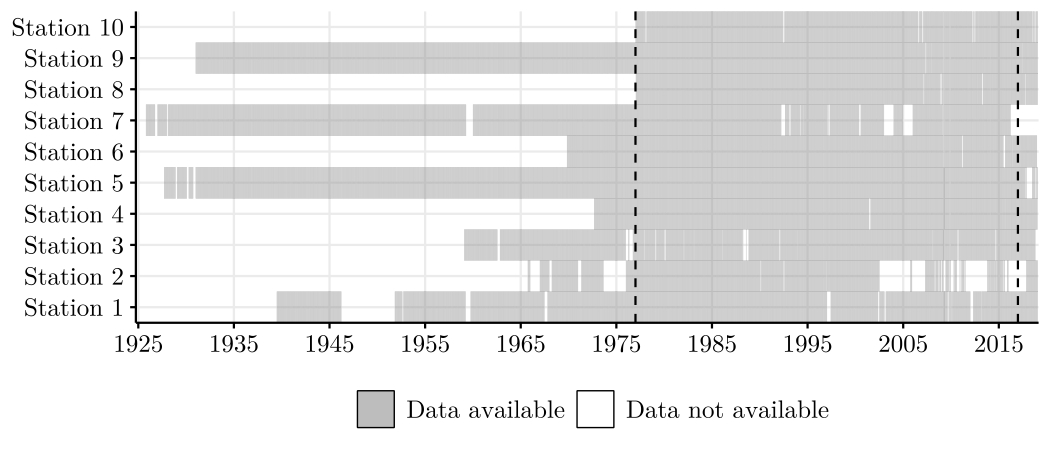
\includegraphics[width=0.7\linewidth,height=\textheight,keepaspectratio]{images/sim/SF_NAdata.jpg}
\end{center}

\subsection{São Francisco River:
Data}\label{suxe3o-francisco-river-data-3}

The study analyzes water volume interactions across \(d=10\) stations
along the river's course.

\textbf{Data Characteristics}:

\begin{itemize}
\tightlist
\item
  Vector \(\mathbf{X}\) observed at 10-day mean discrete intervals.
\item
  Period: Jan 1977 -- Dec 2016 (\(n=1042\) observations).
\item
  \textbf{Discretization}: Five levels based on quantiles.
\end{itemize}

\begin{center}
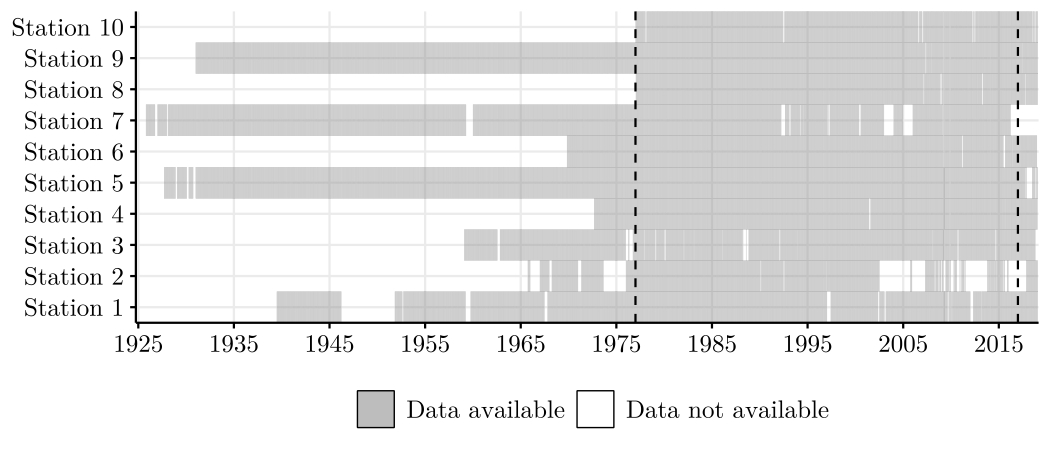
\includegraphics[width=1\linewidth,height=\textheight,keepaspectratio]{images/sim/SF_NAdata.jpg}
\end{center}

\subsection{São Francisco River: Structural
Results}\label{suxe3o-francisco-river-structural-results}

We applied the \textbf{Forward Stepwise Algorithm} with \textbf{5-fold
cross-validation} to select the optimal penalty \(c\).

\paragraph{Physical Network}\label{physical-network}

\begin{center}
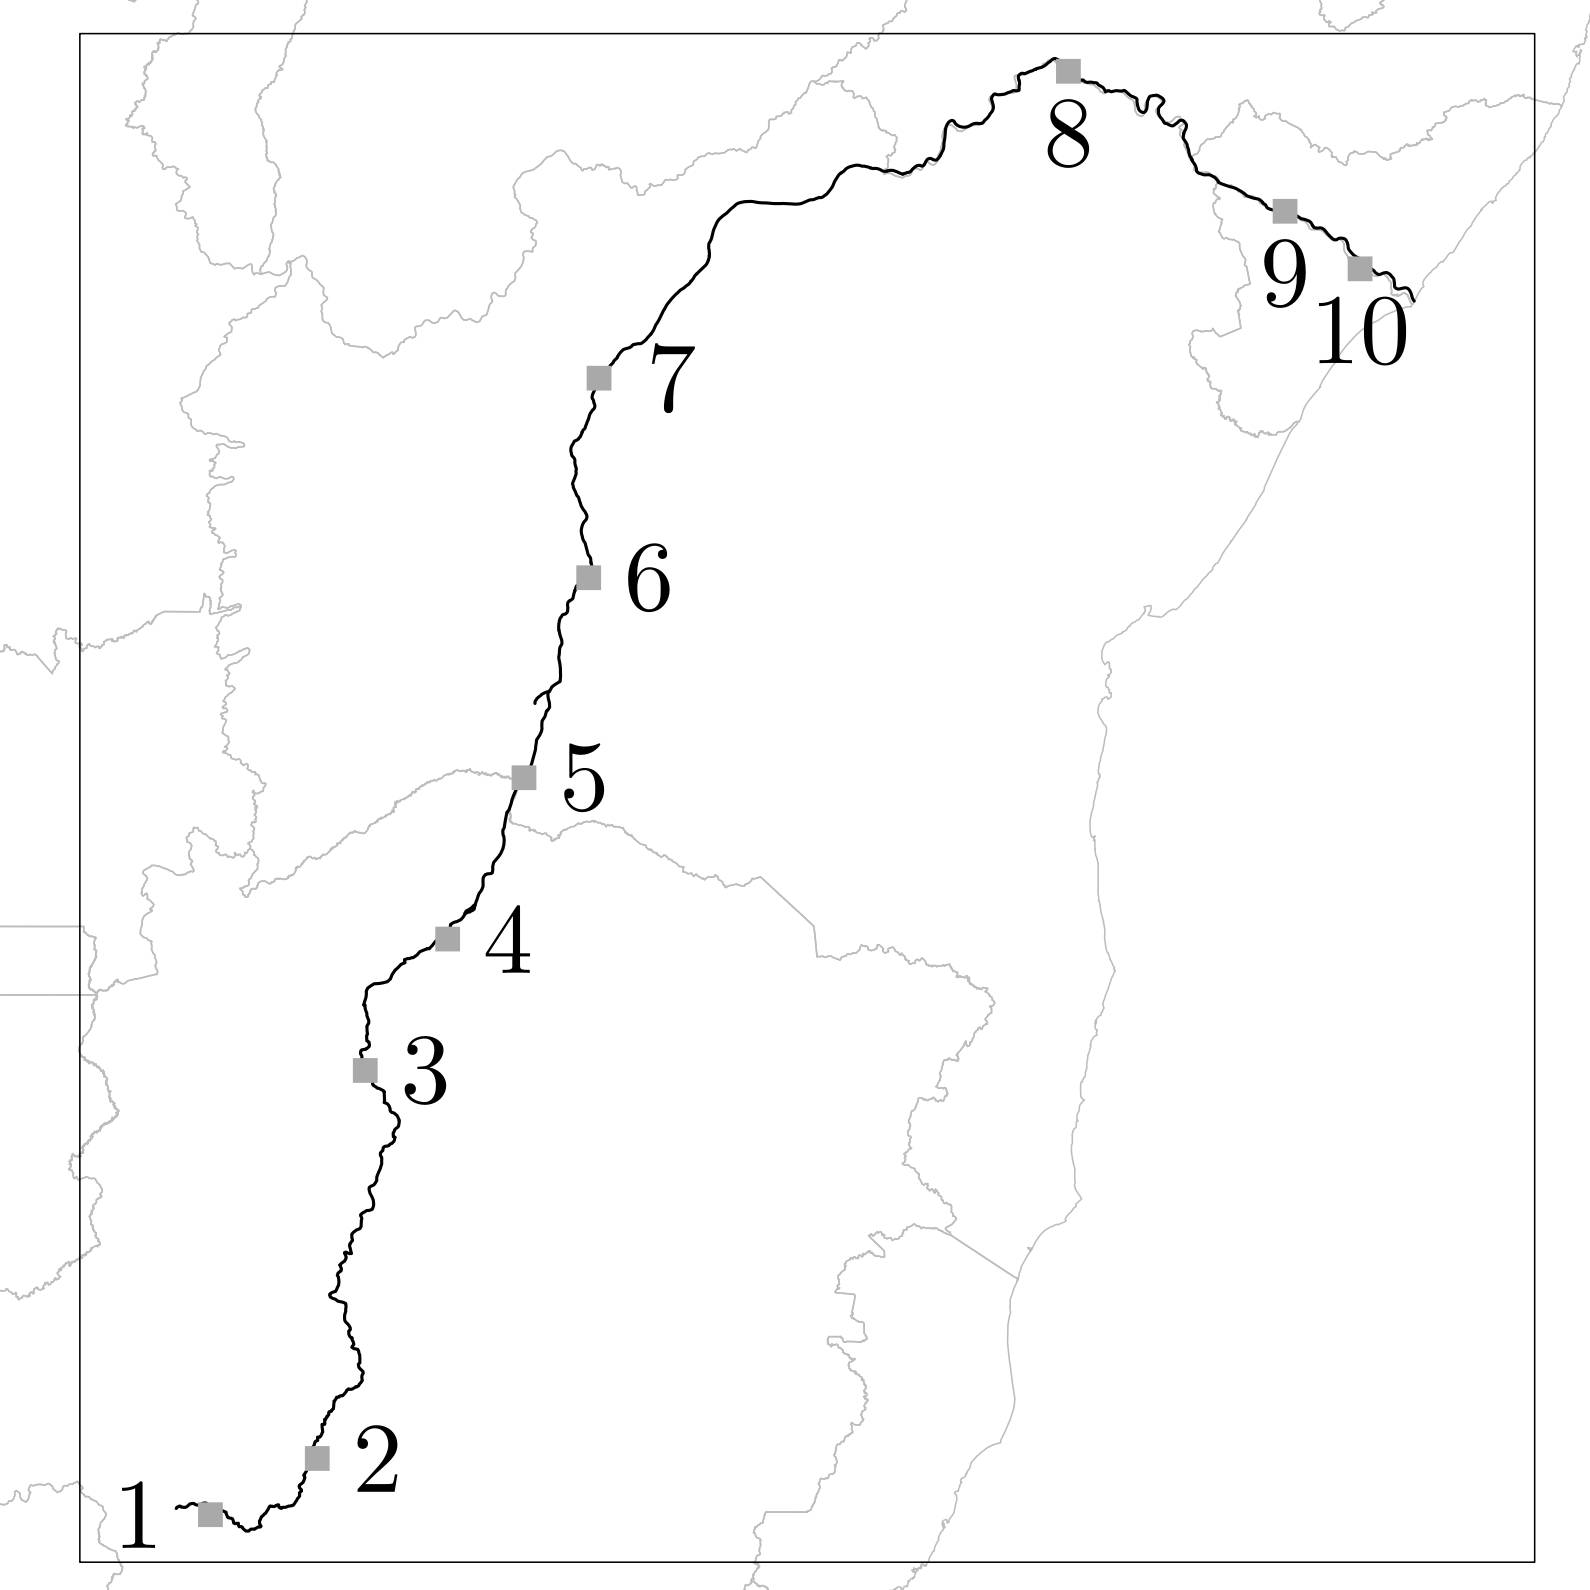
\includegraphics[width=0.65\linewidth,height=\textheight,keepaspectratio]{images/sim/SF_stations.jpg}
\end{center}

\paragraph{\texorpdfstring{Estimated Graph
\(\widehat{G}\)}{Estimated Graph \textbackslash widehat\{G\}}}\label{estimated-graph-widehatg}

\begin{center}
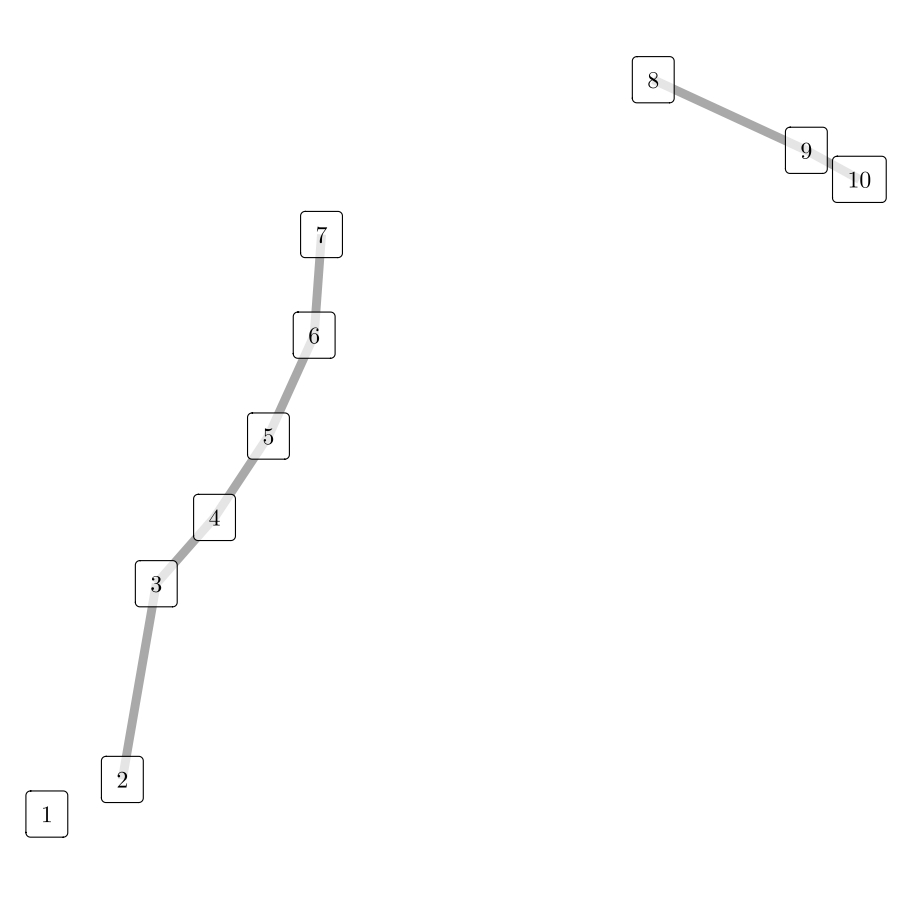
\includegraphics[width=0.65\linewidth,height=\textheight,keepaspectratio]{images/sim/SF_map_best_cv_fwd_N_1042_c_0.4.jpg}
\end{center}

\begin{itemize}
\tightlist
\item
  The estimated edges accurately recover the hydrological flow and
  physical connectivity of the river.
\item
  Results are consistent with independent block identification methods
  (Leonardi et al, 2021).
\end{itemize}

\subsection{Discussion \& Future Work}\label{discussion-future-work}

\begin{itemize}
\tightlist
\item
  \textbf{Summary}:

  \begin{itemize}
  \tightlist
  \item
    Generalization of structure recovery for multivariate processes
    under \textbf{polynomial mixing conditions}.
  \item
    Development of a \textbf{global estimation criterion} based on
    penalized log-pseudo-likelihood.
  \item
    Proved \textbf{strong consistency} and derived convergence rates for
    the estimator \(\widehat{G}\).
  \item
    Implementation of exhaustive and heuristic search algorithms
    (Stepwise, Simulated Annealing).
  \item
    Validation through extensive simulations and applications to
    \textbf{hydrological} and \textbf{financial} data.
  \end{itemize}
\item
  \textbf{Future Directions}:

  \begin{itemize}
  \tightlist
  \item
    Generalization to \textbf{infinite vertex sets} and unbounded degree
    estimators.
  \item
    Extension to \textbf{continuous-valued} multivariate stochastic
    processes.
  \item
    Adaptation of the framework for \textbf{directed graph estimation}
    (causality).
  \end{itemize}
\end{itemize}

\subsection{References}\label{references}

\begin{itemize}
\item
  Cerqueira et al.(2017) Andressa Cerqueira, Daniel Fraiman, Claudia D.
  Vargas and Florencia Leonardi. \textbf{A test of hypotheses for random
  graph distributions built from eeg data}. \emph{IEEE Transactions on
  Network Science and Engineering}, 4(2):75-82.
\item
  Galves et al.(2015) Antonio Galves, Enza Orlandi and Daniel Y.
  Takahashi. \textbf{Identifying interacting pairs of sites in Ising
  models on a countable set}. \emph{Braz. J. Probab. Stat.},
  29(2):443-459.
\item
  Lauritzen(1996) Steffen L Lauritzen. \textbf{Graphical models}, volume
  17. \emph{Clarendon Press}.
\item
  Leonardi et al.(2021) Florencia Leonardi, Matías Lopez-Rosenfeld,
  Daniela Rodriguez, Magno TF Severino and Mariela Sued.
  \textbf{Independent block identification in multivariate time series}.
  \emph{Journal of Time Series Analysis}, 42(1):19-33.
\item
  Leonardi et al.(2023) Florencia Leonardi, Rodrigo Carvalho and Iara
  Frondana. \textbf{Structure recovery for partially observed discrete
  markov random fields on graphs under not necessarily positive
  distributions}. \emph{Scandinavian Journal of Statistics}.
\item
  Meinshausen and Bühlmann(2006) N. Meinshausen and P. Bühlmann.
  \textbf{Highdimensional graphs and variable selection with the lasso}.
  \emph{Ann. Statist.}, 34(3):1436-1462.
\item
  Ravikumar et al.(2010) Pradeep Ravikumar, Martin J. Wainwright and
  John D. Lafferty. \textbf{High-dimensional Ising model selection using
  l1-regularized logistic regression}. \emph{Ann. Statist.},
  38(3):3022-1319.
\end{itemize}

\subsection{}\label{section}

Thank you!

Obrigado!

¡Gracias!




\end{document}
